
%% bare_jrnl.tex
%% V1.3
%% 2007/01/11
%% by Michael Shell
%% see http://www.michaelshell.org/
%% for current contact information.
%%
%% This is a skeleton file demonstrating the use of IEEEtran.cls
%% (requires IEEEtran.cls version 1.7 or later) with an IEEE journal paper.
%%
%% Support sites:
%% http://www.michaelshell.org/tex/ieeetran/
%% http://www.ctan.org/tex-archive/macros/latex/contrib/IEEEtran/
%% and
%% http://www.ieee.org/



% *** Authors should verify (and, if needed, correct) their LaTeX system  ***
% *** with the testflow diagnostic prior to trusting their LaTeX platform ***
% *** with production work. IEEE's font choices can trigger bugs that do  ***
% *** not appear when using other class files.                            ***
% The testflow support page is at:
% http://www.michaelshell.org/tex/testflow/


%%*************************************************************************
%% Legal Notice:
%% This code is offered as-is without any warranty either expressed or
%% implied; without even the implied warranty of MERCHANTABILITY or
%% FITNESS FOR A PARTICULAR PURPOSE! 
%% User assumes all risk.
%% In no event shall IEEE or any contributor to this code be liable for
%% any damages or losses, including, but not limited to, incidental,
%% consequential, or any other damages, resulting from the use or misuse
%% of any information contained here.
%%
%% All comments are the opinions of their respective authors and are not
%% necessarily endorsed by the IEEE.
%%
%% This work is distributed under the LaTeX Project Public License (LPPL)
%% ( http://www.latex-project.org/ ) version 1.3, and may be freely used,
%% distributed and modified. A copy of the LPPL, version 1.3, is included
%% in the base LaTeX documentation of all distributions of LaTeX released
%% 2003/12/01 or later.
%% Retain all contribution notices and credits.
%% ** Modified files should be clearly indicated as such, including  **
%% ** renaming them and changing author support contact information. **
%%
%% File list of work: IEEEtran.cls, IEEEtran_HOWTO.pdf, bare_adv.tex,
%%                    bare_conf.tex, bare_jrnl.tex, bare_jrnl_compsoc.tex
%%*************************************************************************

% Note that the a4paper option is mainly intended so that authors in
% countries using A4 can easily print to A4 and see how their papers will
% look in print - the typesetting of the document will not typically be
% affected with changes in paper size (but the bottom and side margins will).
% Use the testflow package mentioned above to verify correct handling of
% both paper sizes by the user's LaTeX system.
%
% Also note that the "draftcls" or "draftclsnofoot", not "draft", option
% should be used if it is desired that the figures are to be displayed in
% draft mode.
%
\documentclass[journal]{journal}
%
% If IEEEtran.cls has not been installed into the LaTeX system files,
% manually specify the path to it like:
% \documentclass[journal]{../sty/IEEEtran}





% Some very useful LaTeX packages include:
% (uncomment the ones you want to load)


% *** MISC UTILITY PACKAGES ***
%
%\usepackage{ifpdf}
% Heiko Oberdiek's ifpdf.sty is very useful if you need conditional
% compilation based on whether the output is pdf or dvi.
% usage:
% \ifpdf
%   % pdf code
% \else
%   % dvi code
% \fi
% The latest version of ifpdf.sty can be obtained from:
% http://www.ctan.org/tex-archive/macros/latex/contrib/oberdiek/
% Also, note that IEEEtran.cls V1.7 and later provides a builtin
% \ifCLASSINFOpdf conditional that works the same way.
% When switching from latex to pdflatex and vice-versa, the compiler may
% have to be run twice to clear warning/error messages.






% *** CITATION PACKAGES ***
%
%\usepackage{cite}
% cite.sty was written by Donald Arseneau
% V1.6 and later of IEEEtran pre-defines the format of the cite.sty package
% \cite{} output to follow that of IEEE. Loading the cite package will
% result in citation numbers being automatically sorted and properly
% "compressed/ranged". e.g., [1], [9], [2], [7], [5], [6] without using
% cite.sty will become [1], [2], [5]--[7], [9] using cite.sty. cite.sty's
% \cite will automatically add leading space, if needed. Use cite.sty's
% noadjust option (cite.sty V3.8 and later) if you want to turn this off.
% cite.sty is already installed on most LaTeX systems. Be sure and use
% version 4.0 (2003-05-27) and later if using hyperref.sty. cite.sty does
% not currently provide for hyperlinked citations.
% The latest version can be obtained at:
% http://www.ctan.org/tex-archive/macros/latex/contrib/cite/
% The documentation is contained in the cite.sty file itself.






% *** GRAPHICS RELATED PACKAGES ***
\usepackage{tikz}
%\usepackage[outdir=./]{epstopdf}
%\usepackage[pdftex]{graphicx}
%\DeclareGraphicsExtensions{.pdf}
%

% graphicx was written by David Carlisle and Sebastian Rahtz. It is
% required if you want graphics, photos, etc. graphicx.sty is already
% installed on most LaTeX systems. The latest version and documentation can
% be obtained at: 
% http://www.ctan.org/tex-archive/macros/latex/required/graphics/
% Another good source of documentation is "Using Imported Graphics in
% LaTeX2e" by Keith Reckdahl which can be found as epslatex.ps or
% epslatex.pdf at: http://www.ctan.org/tex-archive/info/
%
% latex, and pdflatex in dvi mode, support graphics in encapsulated
% postscript (.eps) format. pdflatex in pdf mode supports graphics
% in .pdf, .jpeg, .png and .mps (metapost) formats. Users should ensure
% that all non-photo figures use a vector format (.eps, .pdf, .mps) and
% not a bitmapped formats (.jpeg, .png). IEEE frowns on bitmapped formats
% which can result in "jaggedy"/blurry rendering of lines and letters as
% well as large increases in file sizes.
%
% You can find documentation about the pdfTeX application at:
% http://www.tug.org/applications/pdftex





% *** MATH PACKAGES ***
%
\usepackage[cmex10]{amsmath}
\usepackage{amsthm}
\usepackage{amssymb}
% A popular package from the American Mathematical Society that provides
% many useful and powerful commands for dealing with mathematics. If using
% it, be sure to load this package with the cmex10 option to ensure that
% only type 1 fonts will utilized at all point sizes. Without this option,
% it is possible that some math symbols, particularly those within
% footnotes, will be rendered in bitmap form which will result in a
% document that can not be IEEE Xplore compliant!
%
% Also, note that the amsmath package sets \interdisplaylinepenalty to 10000
% thus preventing page breaks from occurring within multiline equations. Use:
%\interdisplaylinepenalty=2500
% after loading amsmath to restore such page breaks as IEEEtran.cls normally
% does. amsmath.sty is already installed on most LaTeX systems. The latest
% version and documentation can be obtained at:
% http://www.ctan.org/tex-archive/macros/latex/required/amslatex/math/





% *** SPECIALIZED LIST PACKAGES ***
%
%\usepackage{algorithmic}
% algorithmic.sty was written by Peter Williams and Rogerio Brito.
% This package provides an algorithmic environment fo describing algorithms.
% You can use the algorithmic environment in-text or within a figure
% environment to provide for a floating algorithm. Do NOT use the algorithm
% floating environment provided by algorithm.sty (by the same authors) or
% algorithm2e.sty (by Christophe Fiorio) as IEEE does not use dedicated
% algorithm float types and packages that provide these will not provide
% correct IEEE style captions. The latest version and documentation of
% algorithmic.sty can be obtained at:
% http://www.ctan.org/tex-archive/macros/latex/contrib/algorithms/
% There is also a support site at:
% http://algorithms.berlios.de/index.html
% Also of interest may be the (relatively newer and more customizable)
% algorithmicx.sty package by Szasz Janos:
% http://www.ctan.org/tex-archive/macros/latex/contrib/algorithmicx/




% *** ALIGNMENT PACKAGES ***
%
%\usepackage{array}
% Frank Mittelbach's and David Carlisle's array.sty patches and improves
% the standard LaTeX2e array and tabular environments to provide better
% appearance and additional user controls. As the default LaTeX2e table
% generation code is lacking to the point of almost being broken with
% respect to the quality of the end results, all users are strongly
% advised to use an enhanced (at the very least that provided by array.sty)
% set of table tools. array.sty is already installed on most systems. The
% latest version and documentation can be obtained at:
% http://www.ctan.org/tex-archive/macros/latex/required/tools/


%\usepackage{mdwmath}
%\usepackage{mdwtab}
% Also highly recommended is Mark Wooding's extremely powerful MDW tools,
% especially mdwmath.sty and mdwtab.sty which are used to format equations
% and tables, respectively. The MDWtools set is already installed on most
% LaTeX systems. The lastest version and documentation is available at:
% http://www.ctan.org/tex-archive/macros/latex/contrib/mdwtools/


% IEEEtran contains the IEEEeqnarray family of commands that can be used to
% generate multiline equations as well as matrices, tables, etc., of high
% quality.


%\usepackage{eqparbox}
% Also of notable interest is Scott Pakin's eqparbox package for creating
% (automatically sized) equal width boxes - aka "natural width parboxes".
% Available at:
% http://www.ctan.org/tex-archive/macros/latex/contrib/eqparbox/





% *** SUBFIGURE PACKAGES ***
%\usepackage[tight,footnotesize]{subfigure}
% subfigure.sty was written by Steven Douglas Cochran. This package makes it
% easy to put subfigures in your figures. e.g., "Figure 1a and 1b". For IEEE
% work, it is a good idea to load it with the tight package option to reduce
% the amount of white space around the subfigures. subfigure.sty is already
% installed on most LaTeX systems. The latest version and documentation can
% be obtained at:
% http://www.ctan.org/tex-archive/obsolete/macros/latex/contrib/subfigure/
% subfigure.sty has been superceeded by subfig.sty.



%\usepackage[caption=false]{caption}
%\usepackage[font=footnotesize]{subfig}
% subfig.sty, also written by Steven Douglas Cochran, is the modern
% replacement for subfigure.sty. However, subfig.sty requires and
% automatically loads Axel Sommerfeldt's caption.sty which will override
% IEEEtran.cls handling of captions and this will result in nonIEEE style
% figure/table captions. To prevent this problem, be sure and preload
% caption.sty with its "caption=false" package option. This is will preserve
% IEEEtran.cls handing of captions. Version 1.3 (2005/06/28) and later 
% (recommended due to many improvements over 1.2) of subfig.sty supports
% the caption=false option directly:
%\usepackage[caption=false,font=footnotesize]{subfig}
%
% The latest version and documentation can be obtained at:
% http://www.ctan.org/tex-archive/macros/latex/contrib/subfig/
% The latest version and documentation of caption.sty can be obtained at:
% http://www.ctan.org/tex-archive/macros/latex/contrib/caption/




% *** FLOAT PACKAGES ***
%
%\usepackage{fixltx2e}
% fixltx2e, the successor to the earlier fix2col.sty, was written by
% Frank Mittelbach and David Carlisle. This package corrects a few problems
% in the LaTeX2e kernel, the most notable of which is that in current
% LaTeX2e releases, the ordering of single and double column floats is not
% guaranteed to be preserved. Thus, an unpatched LaTeX2e can allow a
% single column figure to be placed prior to an earlier double column
% figure. The latest version and documentation can be found at:
% http://www.ctan.org/tex-archive/macros/latex/base/



%\usepackage{stfloats}
% stfloats.sty was written by Sigitas Tolusis. This package gives LaTeX2e
% the ability to do double column floats at the bottom of the page as well
% as the top. (e.g., "\begin{figure*}[!b]" is not normally possible in
% LaTeX2e). It also provides a command:
%\fnbelowfloat
% to enable the placement of footnotes below bottom floats (the standard
% LaTeX2e kernel puts them above bottom floats). This is an invasive package
% which rewrites many portions of the LaTeX2e float routines. It may not work
% with other packages that modify the LaTeX2e float routines. The latest
% version and documentation can be obtained at:
% http://www.ctan.org/tex-archive/macros/latex/contrib/sttools/
% Documentation is contained in the stfloats.sty comments as well as in the
% presfull.pdf file. Do not use the stfloats baselinefloat ability as IEEE
% does not allow \baselineskip to stretch. Authors submitting work to the
% IEEE should note that IEEE rarely uses double column equations and
% that authors should try to avoid such use. Do not be tempted to use the
% cuted.sty or midfloat.sty packages (also by Sigitas Tolusis) as IEEE does
% not format its papers in such ways.


%\ifCLASSOPTIONcaptionsoff
%  \usepackage[nomarkers]{endfloat}
% \let\MYoriglatexcaption\caption
% \renewcommand{\caption}[2][\relax]{\MYoriglatexcaption[#2]{#2}}
%\fi
% endfloat.sty was written by James Darrell McCauley and Jeff Goldberg.
% This package may be useful when used in conjunction with IEEEtran.cls'
% captionsoff option. Some IEEE journals/societies require that submissions
% have lists of figures/tables at the end of the paper and that
% figures/tables without any captions are placed on a page by themselves at
% the end of the document. If needed, the draftcls IEEEtran class option or
% \CLASSINPUTbaselinestretch interface can be used to increase the line
% spacing as well. Be sure and use the nomarkers option of endfloat to
% prevent endfloat from "marking" where the figures would have been placed
% in the text. The two hack lines of code above are a slight modification of
% that suggested by in the endfloat docs (section 8.3.1) to ensure that
% the full captions always appear in the list of figures/tables - even if
% the user used the short optional argument of \caption[]{}.
% IEEE papers do not typically make use of \caption[]'s optional argument,
% so this should not be an issue. A similar trick can be used to disable
% captions of packages such as subfig.sty that lack options to turn off
% the subcaptions:
% For subfig.sty:
% \let\MYorigsubfloat\subfloat
% \renewcommand{\subfloat}[2][\relax]{\MYorigsubfloat[]{#2}}
% For subfigure.sty:
% \let\MYorigsubfigure\subfigure
% \renewcommand{\subfigure}[2][\relax]{\MYorigsubfigure[]{#2}}
% However, the above trick will not work if both optional arguments of
% the \subfloat/subfig command are used. Furthermore, there needs to be a
% description of each subfigure *somewhere* and endfloat does not add
% subfigure captions to its list of figures. Thus, the best approach is to
% avoid the use of subfigure captions (many IEEE journals avoid them anyway)
% and instead reference/explain all the subfigures within the main caption.
% The latest version of endfloat.sty and its documentation can obtained at:
% http://www.ctan.org/tex-archive/macros/latex/contrib/endfloat/
%
% The IEEEtran \ifCLASSOPTIONcaptionsoff conditional can also be used
% later in the document, say, to conditionally put the References on a 
% page by themselves.





% *** PDF, URL AND HYPERLINK PACKAGES ***
%
%\usepackage{url}
% url.sty was written by Donald Arseneau. It provides better support for
% handling and breaking URLs. url.sty is already installed on most LaTeX
% systems. The latest version can be obtained at:
% http://www.ctan.org/tex-archive/macros/latex/contrib/misc/
% Read the url.sty source comments for usage information. Basically,
% \url{my_url_here}.





% *** Do not adjust lengths that control margins, column widths, etc. ***
% *** Do not use packages that alter fonts (such as pslatex).         ***
% There should be no need to do such things with IEEEtran.cls V1.6 and later.
% (Unless specifically asked to do so by the journal or conference you plan
% to submit to, of course. )


% correct bad hyphenation here
\hyphenation{op-tical net-works semi-conduc-tor}

\pagestyle{empty}

\begin{document}
	%
	% paper title
	% can use linebreaks \\ within to get better formatting as desired
	\title{Glushkov's construction for functional subsequential transducers}
	%
	%
	% author names and IEEE memberships
	% note positions of commas and nonbreaking spaces ( ~ ) LaTeX will not break
	% a structure at a ~ so this keeps an author's name from being broken across
	% two lines.
	% use \thanks{} to gain access to the first footnote area
	% a separate \thanks must be used for each paragraph as LaTeX2e's \thanks
	% was not built to handle multiple paragraphs
	%
	
	\author{Aleksander Mendoza-Drosik}
	
	
	\newtheorem{theorem}{Theorem}
	\newtheorem{definition}{Definition}
	% note the % following the last \IEEEmembership and also \thanks - 
	% these prevent an unwanted space from occurring between the last author name
	% and the end of the author line. i.e., if you had this:
	% 
	% \author{....lastname \thanks{...} \thanks{...} }
	%                     ^------------^------------^----Do not want these spaces!
	%
	% a space would be appended to the last name and could cause every name on that
	% line to be shifted left slightly. This is one of those "LaTeX things". For
	% instance, "\textbf{A} \textbf{B}" will typeset as "A B" not "AB". To get
	% "AB" then you have to do: "\textbf{A}\textbf{B}"
	% \thanks is no different in this regard, so shield the last } of each \thanks
	% that ends a line with a % and do not let a space in before the next \thanks.
	% Spaces after \IEEEmembership other than the last one are OK (and needed) as
	% you are supposed to have spaces between the names. For what it is worth,
	% this is a minor point as most people would not even notice if the said evil
	% space somehow managed to creep in.
	
	
	
	% The paper headers
	\markboth{Journal of \LaTeX\ Class Files,~Vol.~6, No.~1, January~2007}%
	{Shell \MakeLowercase{\textit{et al.}}: Bare Demo of IEEEtran.cls for Journals}
	% The only time the second header will appear is for the odd numbered pages
	% after the title page when using the twoside option.
	% 
	% *** Note that you probably will NOT want to include the author's ***
	% *** name in the headers of peer review papers.                   ***
	% You can use \ifCLASSOPTIONpeerreview for conditional compilation here if
	% you desire.
	
	
	
	
	% If you want to put a publisher's ID mark on the page you can do it like
	% this:
	%\IEEEpubid{0000--0000/00\$00.00~\copyright~2007 IEEE}
	% Remember, if you use this you must call \IEEEpubidadjcol in the second
	% column for its text to clear the IEEEpubid mark.
	
	
	
	% use for special paper notices
	%\IEEEspecialpapernotice{(Invited Paper)}
	
	
	
	\maketitle
	\thispagestyle{empty}
	
	
	\begin{abstract}
		%\boldmath
		Glushkov's construction has many interesting properties and they become even more evident when applied to transducers. This article strives to show the vast range of possible extensions and optimisations for this algorithm.  Special flavour of regular expressions is introduced, which can be efficiently converted to $\epsilon$-free functional subsequential weighted finite state transducers. Produced automata are very compact, as they contain only one state for each symbol (from input alphabet) of original expression and only one transition for each range of symbols, no matter how large. Such compactified ranges of transitions allow for efficient binary search lookup during automaton evaluation. All the methods and algorithms presented here were used to implement open-source compiler of regular expressions for multitape transducers. 
	\end{abstract}
	% IEEEtran.cls defaults to using nonbold math in the Abstract.
	% This preserves the distinction between vectors and scalars. However,
	% if the journal you are submitting to favors bold math in the abstract,
	% then you can use LaTeX's standard command \boldmath at the very start
	% of the abstract to achieve this. Many IEEE journals frown on math
	% in the abstract anyway.
	
	% Note that keywords are not normally used for peerreview papers.
	\begin{IEEEkeywords}
		weighted automata, transducers, Glushkov, follow automata, regular expressions
	\end{IEEEkeywords}
	
	
	
	
	
	
	% For peer review papers, you can put extra information on the cover
	% page as needed:
	% \ifCLASSOPTIONpeerreview
	% \begin{center} \bfseries EDICS Category: 3-BBND \end{center}
	% \fi
	%
	% For peerreview papers, this IEEEtran command inserts a page break and
	% creates the second title. It will be ignored for other modes.
	\IEEEpeerreviewmaketitle
	
	
	
	\section{Introduction}
	% The very first letter is a 2 line initial drop letter followed
	% by the rest of the first word in caps.
	% 
	% form to use if the first word consists of a single letter:
	% \IEEEPARstart{A}{demo} file is ....
	% 
	% form to use if you need the single drop letter followed by
	% normal text (unknown if ever used by IEEE):
	% \IEEEPARstart{A}{}demo file is ....
	% 
	% Some journals put the first two words in caps:
	% \IEEEPARstart{T}{his demo} file is ....
	% 
	% Here we have the typical use of a "T" for an initial drop letter
	% and "HIS" in caps to complete the first word.
	\IEEEPARstart{T}{here}
 are not many open source solutions available for working with transducers. The most significant and widely used library is OpenFst. Their approach is based on theory of weighted automata\cite{MOHRI3}\cite{DROSTE}\cite{DROSTE2}. Here we propose an alternative approach founded on lexicographic transducers \cite{MendozaDrosik2020MultitapeAA} and Glushkov's algorithm \cite{GLUSHKOV}.


Let $W$ be some set of weight symbols. The free monoid $W^*$ will be out set of weight strings. We assume there is some lexicographic order defined as
\[
b_1w_1 > b_2w_2 \iff w_1 > w_2 \mbox{ or }( w_1=w_2\mbox{ and } b_1 > b_2) \\
\]
where $w_1,w_1\in W$ and $b_1,b_2\in W^*$.  The order is defined only on strings of equal lengths.
Let $\Sigma$ be the input alphabet, $\Sigma^*$ is the monoid of input strings and $D$ is the monoid of output strings.  Lexicographic transducer is defined as tuple $(Q,I,W,\Sigma,D,\delta,\tau)$ where $Q$ is some finite set of states, $I$ is the set of initial states, $\tau$ is a state output (partial) function $Q\rightarrow D \times W$ and lastly $\delta$ represents transitions of the form $\delta \subset Q \times W \times \Sigma \times D \times Q$.

Thanks to $\tau$, such machines are subsequential \cite{MOHRI}\cite{MOHRI2}\cite{HANSAN}\cite{de_la_higuera}. As an example consider the simple transducer from figure \ref{transducer}. The states $q_0$, $q_1$ and $q_2$ have no output, which can be denoted with $\tau(q_0)=\emptyset$. The only set which does have output is $q_3$. Every time automaton finishes reading input string and reaches $q_3$, it will append $d_0$ to its output and then accept. For instance, on input $\sigma_1\sigma_2$ it will first read $\sigma_1$, produce output $d_0d_4$ and go to state $q_1$, then read $\sigma_2$ and append output $d_3$, go to state $q_3$, finally reaching end of input, appending $d_0$ and accepting. The total output would be $d_0d_4d_3d_0$. Note that the automaton is nondeterministic, as it could take alternative route passing through $q_2$ and producing $d_3d_0$. In such scenarios weights are used to disambiguate output. The first route produces weight string $w_2w_3w_1$, while the second produces $w_3w_2w_1$. According to our definition of lexicographic order we have $w_2w_3w_1 > w_3w_2w_1$ (assuming that $w_3>w_2$). Throughout this article we will consider smaller weights to be "better". Hence the automaton should choose $d_3d_0$ as the definitive output for input $\sigma_1\sigma_2$. There might be situations in which two different routes have the exact same (equally highest) weight while also producing different outputs. In such cases, the automaton is ambiguous and produces multiple outputs for one input.


% needed in second column of first page if using \IAENGpubid
%\IAENGpubidadjcol

\section{Expressive power}

There are some remarks to be made about lexicographic transducers.  They recognize relations on languages, unlike "plain" finite state automata (FSA) which recognize languages. If $M$ is some transducer, then we denote its recognized relation with $\mathcal{L}(M)$. Those relations are subsets of $\Sigma^*\times D$. The set of strings $\Sigma^*$ accepted by $M$ must be a regular language (indeed, if we erased output labels, we would as a result obtain FSA). The weights are erasable \cite{MendozaDrosik2020MultitapeAA}  in the sense that, give any lexicographic transducer we can always build an equivalent automaton without weighted transitions. If we didn't have $\tau$, the only output possible to be expressed for empty input would be an empty string as well. With $\tau$ we can express pairs like $(\epsilon,d)\in\mathcal{L}$ where $d\ne\epsilon$.  

The transducers can return at most finitely many outputs for any given input (see \textit{infinite superposition}\cite{MendozaDrosik2020MultitapeAA}). If we allowed for $\epsilon$-transitions (transitions that have $\epsilon$ as input label) we could build $\epsilon$-cycles and produce infinitely many outputs. However, automata that do so are not very interesting from practical point of view. Therefore we shall focus only on functional transducers, that is those which produce at most one output. If automaton does not have any $\epsilon$-cycles and is functional, then it's possible to erase all $\epsilon$-transitions (note that it would not be possible without $\tau$, because $\epsilon$-transitions allow for producing output given empty input). Therefore $\epsilon$-transitions don't increase power of functional transducers.

We say that transducer has \textbf{conflicting states} $q_1$ and $q_2$ if it's possible to reach both of them simultaneously (there are two possible routes with the same inputs and weights) given some input $\sigma$ and there is some another state $q_3$ to which both of those states can transition over the same input symbol $\sigma_i$. Alternatively, there might be no third state $q_3$, but instead both $q_1$ and $q_2$ have non-empty $\tau$ output (so $\tau$ can in a sense be treated like $q_3$). We say that transitions $(q_1,\sigma_i,w,d,q_3)$ and $(q_2,\sigma_i,w',d,q_3)$  are \textbf{weight-conflicting} if they have equal weights $w=w'$.  For instance in figure \ref{transducer} the states $q_1$ and $q_2$ are indeed conflicting because they both transition to $q_3$ over $\sigma_2$ but their transitions are not weight conflicting. It can be shown that transducers without weight-conflicting  transitions are functional. Moreover, if a transducer is functional but contains weight-conflicting transitions, then the weights can be reassigned in such a way that eliminates all conflicts \cite{MendozaDrosik2020MultitapeAA}. The only requirement is that there are enough symbols in $W$ (for instance, if $W$ had only one symbol, then all transitions of conflicting states would always be weight-conflicting). If there are at least as many weight symbols as there are states $\vert W \vert = \vert Q \vert$, then every functional transducer on $\vert W \vert$ states can be built without weight-conflicting transitions. For convenience we can assume that $W=\mathbb{N}$, but in practice all algorithms presented here will work with bounded $W$. Hence transducers without weight-conflicting transitions are equivalent in power to functional transducers. This is important because by searching for weight-conflicting transitions we can efficiently test whether transducer is functional or not.

\section{Ranged automata}


\begin{figure}[!t]
	\centering
	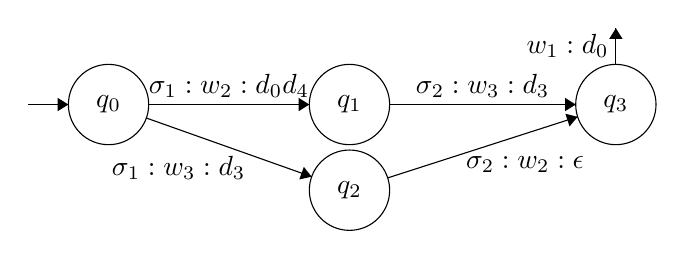
\begin{tikzpicture}[scale=0.17]
	\tikzstyle{every node}+=[inner sep=0pt]
	\draw [black] (18.5,-26.2) circle (3);
	\draw (18.5,-26.2) node {$q_0$};
	\draw [black] (36.5,-26.2) circle (3);
	\draw (36.5,-26.2) node {$q_1$};
	\draw [black] (56.4,-26.2) circle (3);
	\draw (56.4,-26.2) node {$q_3$};
	\draw [black] (36.5,-32.6) circle (3);
	\draw (36.5,-32.6) node {$q_2$};
	\draw [black] (21.5,-26.2) -- (33.5,-26.2);
	\fill [black] (33.5,-26.2) -- (32.7,-25.7) -- (32.7,-26.7);
	\draw (27.5,-25.7) node [above] {$\sigma_1:w_2:d_0d_4$};
	\draw [black] (39.5,-26.2) -- (53.4,-26.2);
	\fill [black] (53.4,-26.2) -- (52.6,-25.7) -- (52.6,-26.7);
	\draw (46.45,-25.7) node [above] {$\sigma_2:w_3:d_3$};
	\draw [black] (21.33,-27.21) -- (33.67,-31.59);
	\fill [black] (33.67,-31.59) -- (33.09,-30.86) -- (32.75,-31.8);
	\draw (23.74,-30.02) node [below] {$\sigma_1:w_3:d_3$};
	\draw [black] (39.36,-31.68) -- (53.54,-27.12);
	\fill [black] (53.54,-27.12) -- (52.63,-26.89) -- (52.94,-27.84);
	\draw (49.61,-30.05) node [below] {$\sigma_2:w_2:\epsilon$};
	\draw [black] (56.4,-23.2) -- (56.4,-20.5);
	\fill [black] (56.4,-20.5) -- (55.9,-21.3) -- (56.9,-21.3);
	\draw (55.9,-21.85) node [left] {$w_1:d_0$};
	\draw [black] (12.5,-26.2) -- (15.5,-26.2);
	\fill [black] (15.5,-26.2) -- (14.7,-25.7) -- (14.7,-26.7);
\end{tikzpicture}
	\caption{Example of lexicographic transducer. State $q_0$ is initial. State $q_3$ in accepting, in the sense that $\tau(q_3)=(w_1,d_0)$. The remaining states have state output $\emptyset$.}
	\label{transducer}
\end{figure}

Often when implementing automata the algorithm behind $\delta$ function needs to efficiently find the right transition for a given $\sigma$ symbol. It's beneficial to optimise UNIX-style ranges like \texttt{[0-9]} or \texttt{[a-z]} as they arise often in practical settings. Even the \texttt{.} wildcard can be treated as one large range spanning entire $\Sigma$. If the alphabet is large (like ASCII or UNICODE), then checking every one of them in a loop is not feasible. A significant improvement can be made by only checking two inequalities like $\sigma_1\le x \le \sigma_{10}$, instead of large number of equalities. The current paper presents a way in which simplified model of $(\mathcal{S},k)$-automata\cite{MEER}\cite{Gandhi}, can be used to obtain major improvements. In particular we consider only automata that don't have any registers apart from constant values, that is $k=0$. Therefore we provide a more specialized definition of "ranged automata". 

Let $\Sigma$ be the (not necessarily finite) alphabet of automaton. Let $\chi$ be the set of subsets of $\Sigma$ that we will call \textbf{ranges} of $\Sigma$. Let  $\overline{\chi}$ be  the closure of $\chi$ under countable union and complementation (so it forms a sigma algebra). For instance, imagine that there is total order on $\Sigma$ and  $\chi$ is the set of all intervals in $\Sigma$. Now we want to build an automaton whose transitions are not labelled with symbols from $\Sigma$, but rather with ranges from $\chi$. Union $\chi_0\cup\chi_1$ of two elements from $\chi$ "semantically" corresponds to putting two edges, $(q,\chi_0,q')\in\delta$ (for a moment forget about outputs and weights) and $(q,\chi_1,q')\in\delta$. There is no limitation on the size of $\delta$. It might be countably infinite, hence it's natural that $\overline{\chi}$ should be closed under countable union. Therefore, $\chi$ is the set of allowed transition labels and $\overline{\chi}$ is the set of all possible "semantic" transitions. We could say that $\overline{\chi}$ is discrete if it contains every subset of $\Sigma$. An example of discrete $\overline{\chi}$ would be finite set $\Sigma$ with all UNIX-style ranges \texttt{[$\sigma$-$\sigma'$]} included in $\chi$. 

Another example would be set $\Sigma=\mathbb{R}$ with $\chi$ consisting of all ranges, whose ends are computable real numbers (real number $x$ is computable if the predicate $q<x$ is decidable for all rational numbers $q$). If we also restricted $\delta$ to be a finite set, then we could build effective automata that work with real numbers of arbitrary precision. 



\section{Regular expressions}

Here we describe a flavour of regular expressions specifically extended to interplay with lexicographic transducers and ranged automata. 

Transducers with input $\Sigma^*$ and output $\Gamma^*$ can be seen as FSA working with single input $\Sigma^* \times \Gamma^*$. Therefore we can treat every pair of symbols $(\sigma,\gamma)$ as an atomic formula of regular expressions for transducers. We can use concatenation $(\sigma,\gamma_0)(\epsilon,\gamma_1)$ to represent $(\sigma,\gamma_0\gamma_1)$. It's possible to create ambiguous transducers with unions like  $(\epsilon,\gamma_0)+(\epsilon,\gamma_1)$.  To make notation easier, we will treat every $\sigma$ as $(\sigma,\epsilon)$ and every $\gamma$ as $(\epsilon,\gamma)$. Then instead of writing lengthy $(\sigma,\epsilon)(\epsilon,\gamma)$ we could introduce shortened notation $\sigma:\gamma$. Because we would like to avoid ambiguous transducers we can put restriction that the right side of $:$ should always be a string of $\Gamma^*$ and writing entire formulas (like $\sigma:\gamma_1+\gamma_2^*$) is not allowed. This restriction will later simplify Glushkov's algorithm. 

We define $\mathcal{A}^\Sigma$ to be the set of atomic characters. For instance we could choose $\mathcal{A}^\Sigma=\Sigma\cup\{\epsilon\}$ for FSA/transducers and $\mathcal{A}^\Sigma=\chi$ for ranged automata. 

We call  $RE^{\Sigma:D}$ the set of all regular expression formulas with underlying set of atomic characters $\mathcal{A}^\Sigma$ and allowed output strings $D$. It's possible that $D$ might be a singleton monoid $\{\epsilon \}$ but it should not be empty, because then no element would belong to $\Sigma^* \times D$. By inductive definition, if $\phi$ and $\psi$  are $RE^{ \Sigma:D}$  formulas and $d \in D$, then union $\phi + \psi$, concatenation $\phi \cdot \psi$, Kleene closure $\phi^*$ and output concatenation $\phi : d$ are $RE^{ \Sigma:D}$ formulas as well.  Define $V^{\Sigma:D}:RE^{\Sigma:D} \rightarrow \Sigma^* \times D$ to be the valuation function:  \\
$V^{\Sigma:D}(\phi + \psi) = V^{\Sigma:D}(\phi) \cup V^{\Sigma:D}(\psi)$ \\
$V^{\Sigma:D}(\phi \cdot \psi) = V^{\Sigma:D}(\phi) \cdot  V^{\Sigma:D}(\psi)$ \\
$V^{\Sigma:D}(\phi^*) = (\epsilon,\epsilon) + V^{\Sigma:D}(\phi) + V^{\Sigma:D}(\phi)^2 + ...$ \\
$V^{\Sigma:D}(\phi : d) = V^{\Sigma:D}(\phi)  \cdot (\epsilon,d)$ \\
$V^{\Sigma:D}(a) = a$ where $a\in\mathcal{A}^{\Sigma:D}$ \\
Some notable properties are: \\
$x:y_0 +x:y_1 = x:(y_0+y_1)$ \\
$x:\epsilon+x:y+x:y^2...=x:y^*$ \\
$(x:y_0)(\epsilon:y_1)  = x:(y_0y_1)$\\
$x_0:(y_0y')+x_1:(y_1y') = (x_0:y_0+x_1:y1)\cdot(\epsilon:y')$ \\
$x_0:(y'y_0)+x_1:(y'y_1) = (\epsilon:y')\cdot(x_0:y_0+x_1:y1)$  \\
Therefore we can see that expressive power with and without $:$ is the same. 

It's also possible to extend regular expressions with weights. Let $RE_W^{\Sigma: D}$ be a superset of $RE^{\Sigma: D}$ and $W$ be the set of weight symbols. If $\phi\in RE_W^{\Sigma\rightarrow D}$ and $w_0,w_1\in W$ then $w_0 \phi $ and  $\phi w_1 $ are in $RE_W^{\Sigma\rightarrow D}$. This allows for inserting weight at any place. For instance, the automaton from figure \ref{transducer} could be expressed using \[
((\sigma_1:d_0d_4)w_2(\sigma_2:d_3)w_3+
(\sigma_1:d_3)w_3\sigma_2w_2):d_0
\]
The definition of $V^{\Sigma:D}(\phi w)$ depends largely on $W$ but associativity $(\phi w_1) w_2 = \phi (w_1 + w_2)$ should be preserved, given that $W$ is a multiplicative monoid. This also implies that $w_1 \epsilon w_2 = w_1 w_2$, which is semantically equivalent to the addition $w_1 + w_2$. 

We showed that regular expressions for transducers can be expressed using pairs of symbols $(\sigma,\gamma)$. There is an alternative approach. We can encode both input and output string by interleaving their symbols like $\sigma_1\gamma_1\sigma_2\gamma_2$. Such regular expressions "recognize" relations rather than "generate" them. This approach has one significant problem. We have to keep track of the order. For instance, this $(\sigma_1\gamma_1\sigma_2 + \sigma_3)\gamma_4$ is a valid interleaved expression but this is not $(\sigma_1\gamma_1 + \sigma_3)\gamma_4$.

In order to decide whether an interleaved regular expression is valid, we should annotate every symbol with its respective alphabet (like $(\sigma_1^\Sigma\gamma_1^\Gamma\sigma_2^\Sigma + \sigma_3^\Sigma)\gamma_4^\Gamma$). Then we rewrite the expression, treating alphabets themselves as the new symbols (for instance $(\Sigma\Gamma\Sigma + \Sigma)\Gamma$). If the language recognized by such expression is a subset of $(\Sigma\Gamma)^*$, then the interleaved expression valid. 

This leads us to introduce \textit{interleaved alphabets}. We should notice that $(\Sigma\Gamma)^*$ is in fact a local language. What it means is that in order to define interleaved alphabet we need 3 sets - set of initial alphabets $U$, set of allowed 2-factors of $V$ and set of final alphabets $W$. Moreover all the elements of $U$ must be pairwise disjoint alphabets. Similarly for $V$ if $(\Sigma_1,\Sigma_2)\in V$ and $(\Sigma_1,\Sigma_3)\in V$  then $\Sigma_2$ and $\Sigma_3$ must be disjoint. (For instance, in case of $(\Sigma\Gamma)^*$  we have $U=\{\Sigma\}$, $V=\{(\Sigma,\Gamma)\}$ and $W=\Gamma$). 

With interleaved alphabets we can encode much more complex "multitape automata". In fact it has certain resemblance to recursive algebraic data structures built from products (like $\{(\Sigma,\Gamma)\}$ in $V$) and coproducts (like $\{(\Sigma,\Gamma_1),(\Sigma,\Gamma_2)\}\in V$) .

It's possible to use interleaved alphabets together with $RE_W^{\Sigma:D}$ to express multitape inputs and mutitape outputs.


\section{Extended Glushkov's construction}

The core result of this paper is Glushkov's algorithm capable of producing very compact, $\epsilon$-free, weighted, ranged, functional, multitape transducers and automatically check if any regular expression is valid, when given specification of interleaved alphabets.

Let $\phi$ be some $RE_W^{\Sigma:D}$ formula. We will call $\Sigma$ the \textit{universal alphabet}. We also admit several subaphabets $\Sigma_1,\Sigma_2,...$ all of which are subsets of $\Sigma$. Each $\Sigma_i$ admits their own set of atomic characters $\mathcal{A}^{\Sigma_i}$ and we require that $\mathcal{A}^{\Sigma_i}\subset \mathcal{A}^{\Sigma}$.  Let $U_\Sigma,V_\Sigma,W_\Sigma$ be the interleaved alphabet consisting of all the subalphabets. For example $\Sigma$ could be the set of all 64-bit integers and then $V_\Sigma$ could contain its subsets like ASCII, UNICODE or binary alphabet $\{0,1\}$ (possibly with offsets to ensure disjointness). In cases when $D=\Gamma^*$, we can similarly define $U_\Gamma,V_\Gamma,W_\Gamma$, but there might be cases where $D$ is more a exotic set (like real numbers) and interleaved alphabet's don't make much sense. Moreover, we require $W$ to be a semiring. For instance, lexicographic weights have concatenation as multiplicative operation and $min$ is used for addition.

First step of Glushkov's algorithm is to create a new alphabet $\Omega$ in which every atomic character (including duplicates but excluding $\epsilon$) in $\phi$ is treated as a new individual character. As a result we should obtain new rewritten formula 
$\psi \in RE_W^{\Omega \rightarrow D} $ along with mapping $\alpha:\Omega \rightarrow\mathcal{A}^\Sigma$. This mapping will remember the original atomic character, before it was rewritten to unique symbol in $\Omega$.
For example 
\[
\phi=(\epsilon:x_0) x_0(x_0:x_1x_3)x_3 w_0+(x_1x_2)^* w_1
\]
will be rewritten as 
\[
\psi=(\epsilon:x_0) \omega_1(\omega_2:x_1x_3)\omega_3 w_0 + (\omega_4\omega_5)^* w_1
\]
with $\alpha= \{(\omega_1,x_0),(\omega_2,x_0),(\omega_3,x_3),(\omega_4,x_1),(\omega_5,x_2)\}$.

Every element $x$ of $\mathcal{A}^\Sigma$ may also be member of several subalphabets. For simplicity we can assume that all expressions are annotated and we know exactly which subalphabet a given $x$ belongs to. In practice, we would try to infer the annotation automatically and ask user to manually annotate symbols only when necessary.

Next step is to define function $\Lambda:RE_W^{\Omega\rightarrow D} \rightharpoonup ( D \times W)$. It returns the output produced for empty word $\epsilon$ (if any) and weight associated with it. (We use symbol $\rightharpoonup$ to highlight the fact that $\Lambda$ is a partial function and may fail for ambiguous transducers.) For instance in the previous example empty word can be matched and the returned output and weight is $(\epsilon,w_1)$. Because both $D$ and $W$ are monoids, we can treat $D \times W$ like a monoid defined as $(y_0,w_0)\cdot(y_1,w_1) = (y_0y_1,w_0+w_1)$. We also admit $\emptyset$ as multiplicative zero, which means that $(y_0,w_0)\cdot\emptyset=\emptyset$. We denote  $W$'s neutral element as $0$. This facilitates recursive definition: \\
$\Lambda(\psi_0+\psi_1) = \Lambda(\psi_0) \cup \Lambda(\psi_1)$ if at least one of the sides is $\emptyset$, otherwise error\\
$\Lambda(\psi_0\psi_1) =\Lambda(\psi_0) \cdot \Lambda(\psi_1)$ \\
$\Lambda(\psi_0 : y) = \Lambda(\psi_0) \cdot (y,0)$ \\
$\Lambda(\psi_0 w) = \Lambda(\psi_0) \cdot (\epsilon,w)$\\
$\Lambda(w \psi_0 ) =  \Lambda(\psi_0) \cdot (\epsilon,w)$ \\
$\Lambda(\psi_0^* ) = (\epsilon,0)$ if $(\epsilon,w) = \Lambda(\psi_0) $ or $\emptyset = \Lambda(\psi_0) $, otherwise error \\
$\Lambda(\epsilon) = (\epsilon,0)$\\
$\Lambda(\omega) = \epsilon$ where $\omega\in\Omega$

Next step is to define $B:RE_W^{\Omega\rightarrow D} \rightarrow (\Omega \rightharpoonup D \times W)$ which for a given formula $\psi$ returns set of $\Omega$ characters that can be found as the first in any string of $V^{\Omega\rightarrow D}(\psi)$ and to each such character we associate output produced "before" reaching it. For instance, in the previous example of $\psi$ there are two characters that can be found at the beginning: $\omega_1$ and $\omega_4$. Additionally, there is $\epsilon$ which prints output $x_0$ before reaching $\omega_1$. Therefore $(\omega_1,(x_0,0))$ and $(\omega_3,(\epsilon,0))$ are the result of $B(\psi)$. For better readability, we admit operation of multiplication $\cdot : (\Omega \rightharpoonup D \times W) \times (D \times W) \rightarrow (\Omega \rightharpoonup D \times W)$ that performs monoid multiplication on all $D \times W$ elements returned by $\Omega \rightharpoonup D \times W$. \\
$B(\psi_0 + \psi_1) = B(\psi_0)\cup B(\psi_1) $ \\
$B(\psi_0 \psi_1) = B(\psi_0) \cup \Lambda(\psi_0)\cdot B(\psi_1)$ \\
$B(\psi_0 w) = B(\psi_0)$ \\
$B(w \psi_0 ) = (\epsilon,w)\cdot B(\psi_0)$ \\
$B(\psi_0^*) =  B(\psi_0)$ \\
$B(\psi_0 : d) =  B(\psi_0)$ \\
$B(\epsilon) =  \emptyset$ \\
$B(\omega) =  \{(\omega,(\epsilon,0)) \}$ \\
It's worth noting that $B(\psi_0)\cup B(\psi_1)$ always yields function  (instead of relation) because every $\Omega$ character appears in $\psi$ only once and it cannot be both in $\psi_0$ and $\psi_1$. 

Next step is to define $E:RE_W^{\Omega\rightarrow D} \rightarrow (\Omega \rightharpoonup D \times W)$, which is very similar to $B$, except that $E$ collects characters found at the end of strings. In our example it would be $(\omega_3,(\epsilon,w_0))$ and $(\omega_5,(\epsilon,w_1))$. Recursive definition is as follows:\\ 
$E(\psi_0 + \psi_1) = E(\psi_0)\cup E(\psi_1) $ \\
$E(\psi_0 \psi_1) = E(\psi_0) \cdot \Lambda(\psi_1) \cup  B(\psi_1)$ \\
$E(\psi_0 w) = E(\psi_0) \cdot (\epsilon,w) $ \\
$E(w \psi_0 ) = E(\psi_0)$ \\
$E(\psi_0 ^*) =  E(\psi_0) $ \\
$E(\psi_0 : d) =  E(\psi_0) \cdot (d,0)$ \\
$E(\epsilon) =  \emptyset$ \\
$E(\omega) =  \{(\omega,(\epsilon,0)) \}$ 

Next step is to use $B$ and $E$ to determine all two-character substrings that can be encountered in $V^{\Omega\rightarrow D}(\psi)$. Given two functions $b,e:\Omega \rightharpoonup D \times W$ we define product $b \times e : \Omega \times \Omega \rightharpoonup  D \times W$ such that for any $(\omega_0,(y_0,w_0))\in b$ and $(\omega_1,(y_1,w_1)) \in c$ there is $((\omega_0,\omega_1),(y_0y_1,w_0+w_1)) \in b\times e$. Then define $L:RE_W^{\Omega\rightarrow D} \rightarrow (\Omega \times \Omega \rightharpoonup  D \times W)$ as: \\
$L(\psi_0 + \psi_1) = L(\psi_0)\cup L(\psi_1) $ \\
$L(\psi_0 \psi_1) = L(\psi_0) \cup  L(\psi_1) \cup E(\psi_0) \times B(\psi_1)$ \\
$L(\psi_0 w) = L(\psi_0) $ \\
$L(w \psi_0 ) = L(\psi_0)$ \\
$L(\psi_0 ^*) =  L(\psi_0) \cup E(\psi_0) \times B(\psi_0)$ \\
$L(\psi_0 : d) =  L(\psi_0)$ \\
$L(\epsilon) =  \emptyset$ \\
$L(\omega) =  \emptyset$  \\
One should notice that all the partial functions produced by $B$, $E$ and $L$ have finite domains, therefore they are effective objects from computational point of view. 

The last step is to use results of $L,B,E,\Lambda$ and $\alpha$ to produce automaton $(Q,q_\epsilon,W,\Sigma,D,\delta,\tau)$ with \\
$\delta:Q \times \Sigma \rightarrow (Q\rightharpoonup D\times W)$ \\
$\tau:Q\rightharpoonup D \times W$ \\
$Q = \{q_\omega : \omega \in \Omega \} \cup \{q_\epsilon\}$ \\
$\tau = E(\psi)$ \\
$(q_{\omega_0},\alpha(\omega_1),q_{\omega_1},d,w)  \in \delta$ for every $(\omega_0,\omega_1,d,w) \in L(\psi) $ \\
$(q_\epsilon,\alpha(\omega),q_{\omega},d,w)  \in \delta$ for every $(\omega,d,w) \in B(\psi) $ 

This concludes the Glushkov's construction. Now it's possible to use specification $U_\Sigma$, $V_\Sigma$ and $W_\Sigma$ of interleaved alphabet to check if regular expression was correct. We can treat alphabets $\Sigma_1,\Sigma_2,...$ as colours and then colour each state with it's respective alphabet. If transition leads from state of colour $\Sigma_i$ to $\Sigma_j$ then we check that the pair $(\Sigma_i,\Sigma_j)$ is indeed present in $V_\Sigma$. Similarly we check colours of initial and accepting states.

\section{Optimisations}

The above construction can detect some obvious cases of ambiguous transducers, but it doesn't give us complete guarantee. We can check in quadratic time\cite{Marie-Pierre} for weight conflicting transitions to be sure. If there are none, then transducer must be functional. If we find at least one, it doesn't immediately imply that the transducer is ambiguous. In such cases we can warn the user and demand additional weight annotations in the regular expression. 

When $\mathcal{A}^\Sigma$ consists of all possible ranges  $\chi$, then the obtained $\delta$ is of the form $Q\times  W \times \chi \times D \times Q$. While, theoretically equivalent to $Q\times  W \times \Sigma \times D \times Q$, in practice it allows for more efficient implementations. For instance given two ranges \texttt{[1-50]} and \texttt{[20-80]}, we do not need to check equality for all $80$ numbers. The only points worth checking are $1,50,20,80$. Let's arrange them in some sorted array. Then given any number $x$, we can use binary search to find which of those points is closest to $x$ and then lookup the full list of intervals that $x$ is a member of. This approach works even for real numbers. More precise algorithm can be given a follows. Let $(x_0,y_0),(x_1,y_1),...(x_n,y_n)$ be closed ranges. Build an array \texttt{P} sorted in ascending order that contains all $y_i$ and also for every $x_i$ contains the largest element of $\Sigma$ smaller than $x_i$ (or more generally the supremum). Build a second array \texttt{R} that to every $i^{th}$ element of \texttt{R} assign list of ranges containing  $i^{th}$ element of \texttt{P}. Then in order to find ranges containing any $x$, run binary search on \texttt{P} that returns index of the largest element smaller or equal to $x$. Then lookup the list of ranges in \texttt{R}. 



In Glushkov's construction epsilons are not rewritten to $\Omega$, which means that there are also no $\epsilon$-transitions. Hence we can use dynamic programming to efficiently evaluate automaton for any input string $x\in\Sigma^*$. The algorithm is as follows. Create two dimensional array $c_{i,j}$ of size $\vert Q \vert \times (\vert x \vert+1)$
where $i$-th column represents all nondeterministically reached states after reading first $i-1$ symbols. Each cell should hold information about the previously used transition. This also tells us the weight, output and source state of transition. For instance cell $c_{i,j}=k$ should encode transition coming from state $k$ to state $i$, after reading $j-1^{th}$ symbol. If state $q_i\in Q$ does not belong to $j^{th}$ superposition, then $c_{i,j}=\emptyset$. The first column is initialized with arbitrary value at $c_{i,1}=-1$ for $i$ referring to initial state $q_\epsilon$ and set to $c_{i,1}=\emptyset$ for all other $i$. Then algorithm progresses building next column from previous one. After filling out the entire array. The last column should be checked for any accepting states according to $\tau$. There might be many of them but the one with largest weight should be chosen. If we checked that the automaton has no weight-conflicting transitions, then there should always be only one maximal weight. Finally we can backtrack, to find out which path "won". This will determine what outputs need to be concatenated together to obtain path's output. This algorithm is quadratic $O(\vert Q\vert, \vert x \vert)$, but in practice each iteration itself is very efficient, especially when combined with binary search described in previous paragraph. By observing that states of automata are often sparsely connected, additional optimisation can be made by representing the two dimensional array with list of indices, as it's often done for sparse matrices.







% An example of a floating figure using the graphicx package.
% Note that \label must occur AFTER (or within) \caption.
% For figures, \caption should occur after the \includegraphics.
% Note that IAENGtran v1.7 and later has special internal code that
% is designed to preserve the operation of \label within \caption
% even when the captionsoff option is in effect. However, because
% of issues like this, it may be the safest practice to put all your
% \label just after \caption rather than within \caption{}.
%
% Reminder: the "draftcls" or "draftclsnofoot", not "draft", class
% option should be used if it is desired that the figures are to be
% displayed while in draft mode.
%
%\begin{figure}[!t]
%\centering
%\includegraphics[width=2.5in]{myfigure}
% where an .eps filename suffix will be assumed under latex,
% and a .pdf suffix will be assumed for pdflatex; or what has been declared
% via \DeclareGraphicsExtensions.
%\caption{Simulation Results}
%\label{fig_sim}
%\end{figure}





% Note that IAENG does not put floats in the very first column - or typically
% anywhere on the first page for that matter. Also, in-text middle ("here")
% positioning is not used. Most IAENG journals use top floats exclusively.
% Note that, LaTeX2e, unlike IAENG journals, places footnotes above bottom
% floats. This can be corrected via the \fnbelowfloat command of the
% stfloats package.



\section{Conclusion}

Interleaved alphabets could find numerous applications with many possible extensions. In the context of natural language processing, they could be used to annotate human sentences with linguistic meta-information like parts of speech. Then transducers could built to take advantage of those tag. Using grammatical inference methods, one could also train such transducers to as POS taggers.

This approach cannot fully replace OpenFST, because it lacks their flexibility. The goal of OpenFST is to provide general and extensible implementation of many different transducer's, whereas the approach presented in this paper sacrifices extensibility for highly integrated design and optimal efficiency. For instance, Glushkov's algorithm could never support such operations  as inverses, projections, reverses or composition. 


% if have a single appendix:
%\appendix[Proof of the Zonklar Equations]
% or
%\appendix  % for no appendix heading
% do not use \section anymore after \appendix, only \section*
% is possibly needed

% use appendices with more than one appendix
% then use \section to start each appendix
% you must declare a \section before using any
% \subsection or using \label (\appendices by itself
% starts a section numbered zero.)
%



% use section* for acknowledgement
\section*{Acknowledgment}


The authors would like to thank Piotr Radwan for all the inspiration.

	
	
	
	% trigger a \newpage just before the given reference
	% number - used to balance the columns on the last page
	% adjust value as needed - may need to be readjusted if
	% the document is modified later
	%\IEEEtriggeratref{8}
	% The "triggered" command can be changed if desired:
	%\IEEEtriggercmd{\enlargethispage{-5in}}
	
	% references section
	
	% can use a bibliography generated by BibTeX as a .bbl file
	% BibTeX documentation can be easily obtained at:
	% http://www.ctan.org/tex-archive/biblio/bibtex/contrib/doc/
	% The IEEEtran BibTeX style support page is at:
	% http://www.michaelshell.org/tex/ieeetran/bibtex/
	%\bibliographystyle{IEEEtran}
	% argument is your BibTeX string definitions and bibliography database(s)
	%\bibliography{IEEEabrv,../bib/paper}
	%
	% <OR> manually copy in the resultant .bbl file
	% set second argument of \begin to the number of references
	% (used to reserve space for the reference number labels box)
	
	
	% biography section
	% 
	% If you have an EPS/PDF photo (graphicx package needed) extra braces are
	% needed around the contents of the optional argument to biography to prevent
	% the LaTeX parser from getting confused when it sees the complicated
	% \includegraphics command within an optional argument. (You could create
	% your own custom macro containing the \includegraphics command to make things
	% simpler here.)
	%\begin{biography}[{\includegraphics[width=1in,height=1.25in,clip,keepaspectratio]{mshell}}]{Michael Shell}
	% or if you just want to reserve a space for a photo:
	
	\bibliographystyle{BibTeXtran}   % (uses file "BibTeXtran.bst")
	\bibliography{BibTeXrefs}       % (expects the reference in the file "BibTeXrefs.bib")
	
	
	% You can push biographies down or up by placing
	% a \vfill before or after them. The appropriate
	% use of \vfill depends on what kind of text is
	% on the last page and whether or not the columns
	% are being equalized.
	
	%\vfill
	
	% Can be used to pull up biographies so that the bottom of the last one
	% is flush with the other column.
	%\enlargethispage{-5in}
	
	
	
	% that's all folks
\end{document}


